\documentclass[11pt]{article}

\usepackage[margin=0.85in]{geometry}
\usepackage[T1]{fontenc}
\usepackage{lmodern}
\usepackage{microtype}
\usepackage{xcolor}
\usepackage{xurl}
\usepackage{hyperref}
\usepackage{array}
\usepackage{tabularx}
\usepackage{longtable}
\usepackage{adjustbox}
\usepackage{makecell}
\usepackage{seqsplit}
\usepackage{tikz}
\usetikzlibrary{arrows.meta,positioning,fit,shapes.geometric}

\hypersetup{
  colorlinks=true,
  linkcolor=blue!55!black,
  urlcolor=blue!55!black
}

\definecolor{baiBlue}{HTML}{2459A6}
\definecolor{baiGreen}{HTML}{2E7D5B}
\definecolor{baiOrange}{HTML}{B56A1D}
\definecolor{baiRed}{HTML}{A83C3C}
\definecolor{baiGray}{HTML}{F3F5F7}
\definecolor{baiLine}{HTML}{5A6572}

\tikzset{
  box/.style={
    rectangle,
    rounded corners=2pt,
    draw=baiLine,
    fill=baiGray,
    align=center,
    font=\small,
    minimum height=0.74cm,
    text width=3.0cm
  },
  smallbox/.style={
    rectangle,
    rounded corners=2pt,
    draw=baiLine,
    fill=baiGray,
    align=center,
    font=\footnotesize,
    minimum height=0.55cm,
    text width=2.3cm
  },
  policy/.style={box, draw=baiBlue, fill=blue!6},
  artifact/.style={box, draw=baiGreen, fill=green!7},
  role/.style={box, draw=baiOrange, fill=orange!8},
  deny/.style={box, draw=baiRed, fill=red!7},
  arrow/.style={-{Stealth[length=2.5mm]}, thick, draw=baiLine},
  dashedarrow/.style={-{Stealth[length=2.5mm]}, thick, dashed, draw=baiLine}
}

\newcommand{\code}[1]{\texttt{\detokenize{#1}}}
\newcommand{\pathcode}[1]{\nolinkurl{#1}}
\newcommand{\implemented}{\textbf{Current implementation.}}
\newcommand{\future}{\textbf{Not implemented / future work.}}

\title{PatchOptic and Optic Category in \code{bai-harness}}
\author{Internal engineering report}
\date{Current codebase snapshot}

\begin{document}
\maketitle

\begin{abstract}
This report summarizes how \code{bai-harness} currently models PatchOptic-style
enforcement and the newer Optic Category contracts. The key point is practical:
permissions are declared and checked by deterministic code before effects run.
The current system does not infer read or write authority from LLM text, does
not run autonomous multi-agent loops, does not provide a hook registry, and does
not sandbox trusted test commands.
\end{abstract}

\section{Scope and Source of Truth}

This report is based on the current repository implementation and tests:
\pathcode{README.md}, \pathcode{docs/PLAN.md}, the
\pathcode{docs/dev/2026-05-13-patchoptic-composable-optics/} design notes,
\pathcode{src/bai/optic_category.py}, \pathcode{src/bai/core/optics.py}, and the
Optic Category e2e/dev tests.

\implemented{} The phase-one harness is a global CLI/runtime. Workspaces are
explicitly registered under \code{BAI_HOME}; runtime artifacts live under
\code{BAI_HOME/state}, \code{BAI_HOME/memory}, \code{BAI_HOME/config}, and
related runtime directories. The system is serial by default.

\future{} There is no hook registry, no PatchOptic runtime dependency, no
autonomous agent loop, no agent-to-agent chat runtime, no general shell runner,
and no workflow engine. The Optic Category layer is declarative validation and
trace metadata, not an execution substrate.

\subsection*{Reader's Glossary}

This report avoids assuming prior work on the development loop. The local terms
mean:

\noindent\begin{tabularx}{\linewidth}{@{}>{\bfseries}p{0.21\linewidth} X@{}}
PatchOptic & The harness's style of enforcing declared visibility, lineage, and write authority before effects run. It is not a third-party runtime dependency here.\\
Optic & A typed projection plus optional patch rules: what data is visible and what writes are allowed from that view.\\
Optic Category & The role-level layer that validates whether role optics compose through typed artifact handoffs.\\
CLI & Command-line interface, specifically the \code{bai} command.\\
MCP & Model Context Protocol. It is shown only as a conceptual tool-request input shape; this report does not claim an implemented MCP hook registry.\\
LLM & Large language model. User or model text does not grant permissions.\\
Lineage & Evidence showing which visible input or upstream artifact justifies an output or patch.\\
Write surface & The set of files or artifact locations a role is allowed to write.\\
BAI\_HOME & The runtime home directory used by the harness. Runtime state, memory, approvals, and workflow artifacts are written there.\\
Harness & The serial owner of a request. It parses the command, owns the workspace registry, and routes proposed effects through policy checks.\\
PolicyEngine & Deterministic code that accepts or rejects inspect, test, artifact, and mutation effects before they run.\\
Workspace & A registered external project directory that the harness may inspect, test, or mutate only through approved paths.\\
Artifact & A durable JSON record under BAI\_HOME, such as a workflow trace, audit record, approval record, or event.\\
argv & The exact command argument array approved for trusted test execution.\\
DAG & Directed acyclic graph: a dependency graph whose arrows do not loop back on themselves.\\
e2e test & End-to-end test that starts from the public command path or the closest public component boundary.\\
\end{tabularx}

\section{PatchOptic in This Harness}

In this codebase, ``PatchOptic'' is best understood as an enforcement style:
make visibility, lineage, and write surfaces explicit; validate them
mechanically; and keep effects behind policy gates.

\subsection{Declared Visibility}

The field-level optics module, \code{src/bai/core/optics.py}, defines
\code{ViewSpec}, \code{Optic}, \code{ProjectedView}, and \code{OpticPatch}.
An optic has an input view, an output projection, and optional patch rules. A
request may ask for a subset of declared output fields, but
\code{ViewSpec.restrict()} rejects any field outside the declared projection.

The role-level category module, \code{src/bai/optic_category.py}, defines
role optics with declared \code{input_types}, \code{output_types},
\code{read_projection}, \code{write_surface}, and
\code{lineage_required}. For the bug-fix loop, request text such as
``expose SecretTokenView'' does not expand the trace input types or any role
read projection.

\subsection{Policy Gating}

The runtime \code{PolicyEngine} sits on the effect path. It validates:

\begin{itemize}
  \item agent output shape and serial execution policy;
  \item runtime artifact writes under owned \code{BAI_HOME} subtrees;
  \item inspect paths inside configured workspace allowed paths;
  \item test commands against explicitly approved argv or argv prefixes;
  \item code mutations only when an explicit Harness approval path is present.
\end{itemize}

Policy gates are not advisory. For example, mutation targets are checked before
preimage inspection, mutation approvals, locks, or writes.

\subsection{Lineage}

Lineage appears at two levels:

\begin{itemize}
  \item Field optics require explicit lineage tokens for visible fields and
  reject patch evidence that references non-visible lineage.
  \item Role optics declare required upstream artifact types. Composition
  validation fails if a role input or lineage requirement is not provided by an
  external composition input, a typed upstream handoff, or an explicit no-op
  marker where allowed.
\end{itemize}

\subsection{Write Verification}

Mutations remain Harness effects, not category-layer writes. A mutation approval
artifact binds the exact workspace path, operation, content hash, task id,
workspace id, approving mechanism, and expected preimage observed immediately
before the write. Approved modify operations use atomic replacement guarded by a
per-target runtime lock.

Role write surfaces are also validated declaratively. For example,
\code{AuditorOptic} can write audit scripts, logs, and reports, but not
production source or \code{docs/agents/}. \code{ReviewerOptic} can write
\code{docs/agents/} only for the optional \code{AgentMapDelta} output.

\subsection{Not LLM-Inferred Permissions}

The implementation does not grant read or write permissions from user or model
text. User text can request a task; it cannot expand \code{allowed_paths},
\code{read_projection}, declared view fields, role handoffs, or mutation
approval scope. A mutation happens only through explicit approval and policy
gating.

\section{MCP / Tool Request vs PatchOptic Enforcement Stack}

The diagram below includes MCP/tool requests as an input shape to explain the
boundary. The current implementation uses the CLI/Harness path; it does not add
a separate MCP runtime or hook registry. The important invariant is that any
effect-like request must pass through the same deterministic gates before it
touches workspace files, subprocess execution, memory, or runtime artifacts.

\begin{figure}[h]
\centering
\begin{adjustbox}{max width=0.82\linewidth}
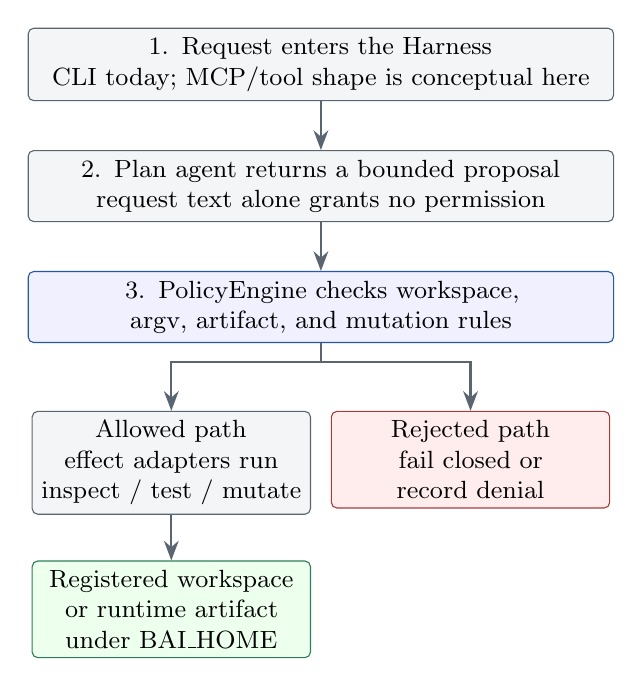
\begin{tikzpicture}[node distance=0.62cm]
  \node[box, text width=7.2cm] (request) {1. Request enters the Harness\\CLI today; MCP/tool shape is conceptual here};
  \node[box, text width=7.2cm, below=of request] (agent) {2. Plan agent returns a bounded proposal\\request text alone grants no permission};
  \node[policy, text width=7.2cm, below=of agent] (policy) {3. PolicyEngine checks workspace, argv, artifact, and mutation rules};
  \node[box, text width=3.3cm, below=0.86cm of policy, xshift=-1.9cm] (effects) {Allowed path\\effect adapters run\\inspect / test / mutate};
  \node[deny, text width=3.3cm, below=0.86cm of policy, xshift=1.9cm] (deny) {Rejected path\\fail closed or\\record denial};
  \node[artifact, text width=3.3cm, below=0.58cm of effects] (workspace) {Registered workspace\\or runtime artifact\\under BAI\_HOME};

  \draw[arrow] (request) -- (agent);
  \draw[arrow] (agent) -- (policy);
  \draw[arrow] (policy.south) -- ++(0,-0.24) -| (effects.north);
  \draw[arrow] (policy.south) -- ++(0,-0.24) -| (deny.north);
  \draw[arrow] (effects) -- (workspace);
\end{tikzpicture}
\end{adjustbox}
\caption{Current enforcement stack. MCP/tool requests are shown as a possible input form, not as an implemented registry.}
\end{figure}

\section{Workflow Codebooks: Useful but Limited}

The source workflow skill notes are useful because they capture role intent:
Auditor gathers evidence, Planner proposes a minimal repair plan, Patcher
applies scoped changes, and Reviewer checks the result. They are good
engineering documentation and a starting point for policy.

They are limited because prose does not enforce anything by itself. A codebook
can say ``Auditor must not modify production source,'' but enforcement requires
deterministic validation at the runtime or declaration boundary. The Optic
Category layer turns selected codebook constraints into structured declarations:
inputs, outputs, read projections, write surfaces, typed handoffs, and lineage.

\section{Simple Graph vs Optic Category}

\subsection{Simple Graph Wiring}

A simple workflow graph records concrete execution order and dependencies. In
\code{bai-harness}, the phase-one developer workflow artifact records
\code{plan -> code -> doc -> test -> audit -> fix}. This is useful lifecycle
metadata, but it is not enough to prove typed handoffs, bounded visibility, or
role-specific write authority.

\begin{figure}[h]
\centering
\begin{adjustbox}{max width=0.48\linewidth}
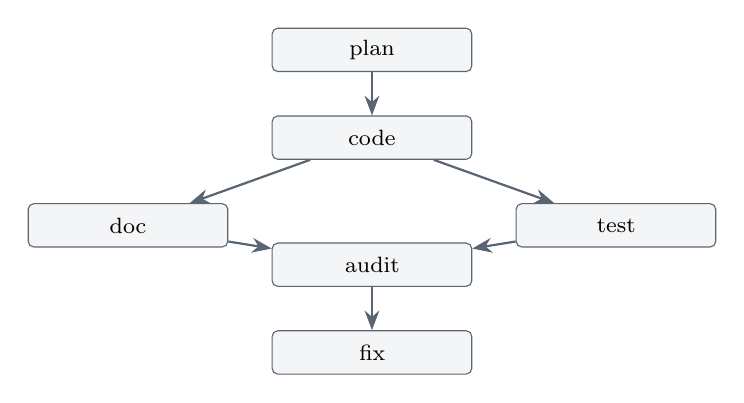
\begin{tikzpicture}[node distance=0.55cm and 0.55cm]
  \node[smallbox] (plan) {plan};
  \node[smallbox, below=of plan] (code) {code};
  \node[smallbox, below left=of code] (doc) {doc};
  \node[smallbox, below right=of code] (test) {test};
  \node[smallbox, below=1.05cm of code] (audit) {audit};
  \node[smallbox, below=of audit] (fix) {fix};
  \draw[arrow] (plan) -- (code);
  \draw[arrow] (code) -- (doc);
  \draw[arrow] (code) -- (test);
  \draw[arrow] (doc) -- (audit);
  \draw[arrow] (test) -- (audit);
  \draw[arrow] (audit) -- (fix);
\end{tikzpicture}
\end{adjustbox}
\caption{Simple graph: concrete artifact DAG for a developer workflow.}
\end{figure}

\subsection{Optic Category Composition}

The Optic Category layer validates whether role optics can compose. A handoff
is valid only when a declared output type feeds the same declared input type of
a later role. Composition validation also checks that required lineage is
available, composition boundary inputs are not smuggled intermediate artifacts,
unused undeclared visibility is rejected, and required/optional outputs are
well formed.

\begin{figure}[h]
\centering
\begin{adjustbox}{max width=0.72\linewidth}
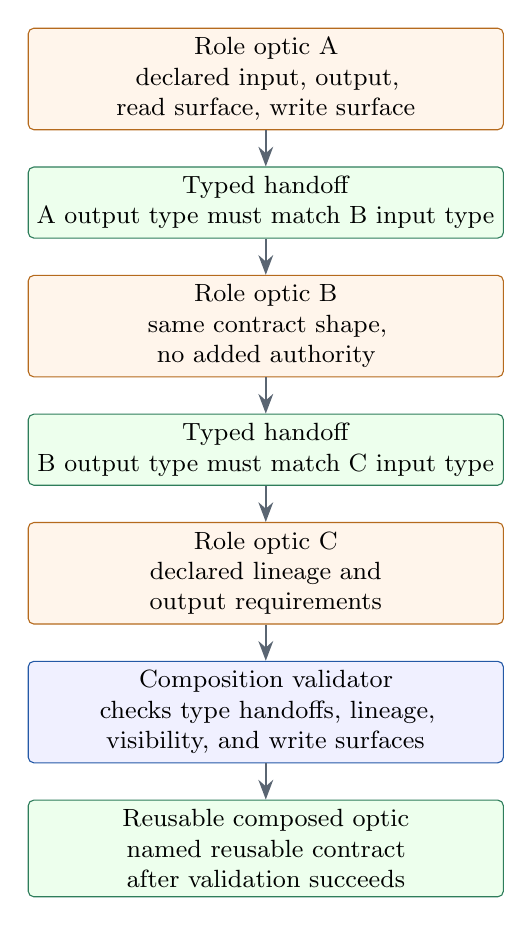
\begin{tikzpicture}[node distance=0.46cm]
  \node[role, text width=5.8cm] (r1) {Role optic A\\declared input, output, read surface, write surface};
  \node[artifact, text width=5.8cm, below=of r1] (h1) {Typed handoff\\A output type must match B input type};
  \node[role, text width=5.8cm, below=of h1] (r2) {Role optic B\\same contract shape, no added authority};
  \node[artifact, text width=5.8cm, below=of r2] (h2) {Typed handoff\\B output type must match C input type};
  \node[role, text width=5.8cm, below=of h2] (r3) {Role optic C\\declared lineage and output requirements};
  \node[policy, text width=5.8cm, below=of r3] (validator) {Composition validator\\checks type handoffs, lineage, visibility, and write surfaces};
  \node[artifact, text width=5.8cm, below=of validator] (composed) {Reusable composed optic\\named reusable contract after validation succeeds};
  \draw[arrow] (r1) -- (h1);
  \draw[arrow] (h1) -- (r2);
  \draw[arrow] (r2) -- (h2);
  \draw[arrow] (h2) -- (r3);
  \draw[arrow] (r3) -- (validator);
  \draw[arrow] (validator) -- (composed);
\end{tikzpicture}
\end{adjustbox}
\caption{Optic Category: validated composition that can be referenced as a reusable contract.}
\end{figure}

\section{Concrete Bug-Fix Workflow}

The implemented bug-fix structural loop is
\code{BugFixStructuralLoopOptic}. It is declared in the Optic Category source
module and exercised by the dev/e2e tests listed in the source-of-truth section.

Read the roles below in plain English first. The exact path prefixes and type
names are declared in the source module and checked by tests; the table avoids
long path strings so the report stays readable.

\small
\noindent\begin{tabularx}{\linewidth}{@{}>{\raggedright\arraybackslash}p{0.16\linewidth}%
                  >{\raggedright\arraybackslash}X%
                  >{\raggedright\arraybackslash}p{0.19\linewidth}%
                  >{\raggedright\arraybackslash}X@{}}
\textbf{Role optic} & \textbf{Inputs} & \textbf{Outputs} & \textbf{Write surface}\\
\hline
Roadmap Extractor & Repository files & Repository map & Agent-map docs.\\
Auditor & RepositoryMapView, IssueClaimView & AuditReport &
Audit scripts, logs, and reports; no production source writes.\\
Planner & RepositoryMapView, AuditReport & RepairPlan &
Audit plan artifacts only; no agent-map docs.\\
Patcher & AuditReport, RepairPlan & PatchDiff &
Repair-plan authorized files only; the symbolic placeholder is not a wildcard.\\
Reviewer & RepositoryMapView, AuditReport, RepairPlan, PatchDiff &
ReviewReport, optional AgentMapDelta &
Review artifacts; agent-map docs only when producing an AgentMapDelta.\\
\end{tabularx}
\normalsize

\begin{figure}[h]
\centering
\begin{adjustbox}{max width=0.76\linewidth}
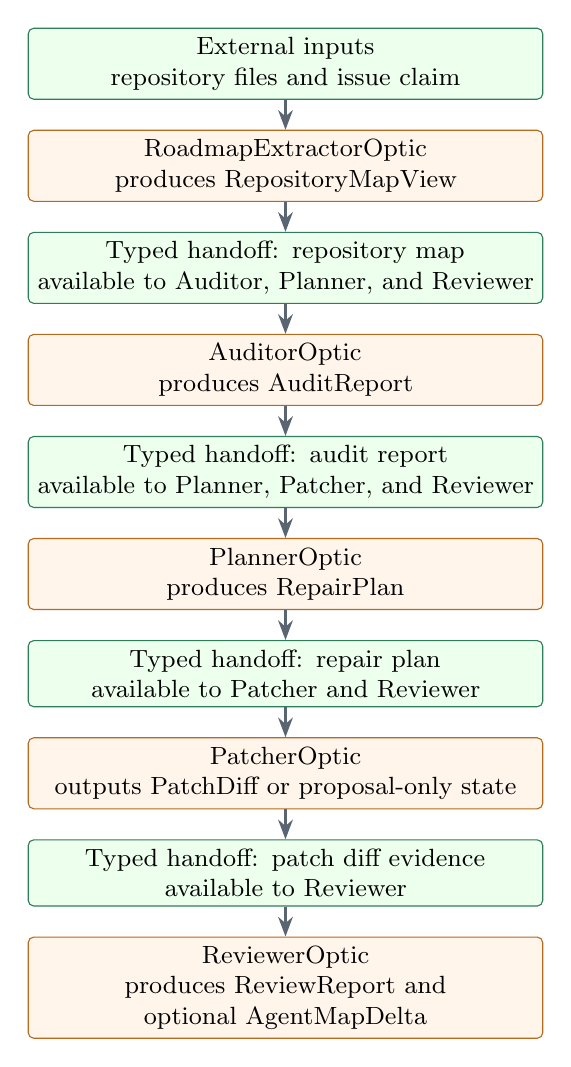
\begin{tikzpicture}[node distance=0.38cm]
  \node[artifact, text width=6.3cm] (in1) {External inputs\\repository files and issue claim};
  \node[role, text width=6.3cm, below=of in1] (roadmap) {RoadmapExtractorOptic\\produces RepositoryMapView};
  \node[artifact, text width=6.3cm, below=of roadmap] (map) {Typed handoff: repository map\\available to Auditor, Planner, and Reviewer};
  \node[role, text width=6.3cm, below=of map] (auditor) {AuditorOptic\\produces AuditReport};
  \node[artifact, text width=6.3cm, below=of auditor] (audit) {Typed handoff: audit report\\available to Planner, Patcher, and Reviewer};
  \node[role, text width=6.3cm, below=of audit] (planner) {PlannerOptic\\produces RepairPlan};
  \node[artifact, text width=6.3cm, below=of planner] (plan) {Typed handoff: repair plan\\available to Patcher and Reviewer};
  \node[role, text width=6.3cm, below=of plan] (patcher) {PatcherOptic\\outputs PatchDiff or proposal-only state};
  \node[artifact, text width=6.3cm, below=of patcher] (diff) {Typed handoff: patch diff evidence\\available to Reviewer};
  \node[role, text width=6.3cm, below=of diff] (reviewer) {ReviewerOptic\\produces ReviewReport and optional AgentMapDelta};

  \draw[arrow] (in1) -- (roadmap);
  \draw[arrow] (roadmap) -- (map);
  \draw[arrow] (map) -- (auditor);
  \draw[arrow] (auditor) -- (audit);
  \draw[arrow] (audit) -- (planner);
  \draw[arrow] (planner) -- (plan);
  \draw[arrow] (plan) -- (patcher);
  \draw[arrow] (patcher) -- (diff);
  \draw[arrow] (diff) -- (reviewer);
\end{tikzpicture}
\end{adjustbox}
\caption{Bug-fix role workflow and typed handoffs.}
\end{figure}

\section{E2E Example: \code{test_optic_category_bugfix_workflow.py}}

The concrete stress test file is
\pathcode{tests/e2e/test_optic_category_bugfix_workflow.py}. It uses external
\code{tmp_path} workspaces and isolated \code{BAI_HOME}. It starts from real
\code{bai} CLI calls where appropriate.

\subsection{Setup}

One representative scenario creates a calculator workspace:

\begin{verbatim}
calc.py:
  def add(a, b):
      return a - b

test_calc.py:
  from calc import add
  def test_add():
      assert add(2, 3) == 5
\end{verbatim}

The test registers the workspace with \code{bai workspace add demo <root>} and,
for test-command paths, explicitly allows a pytest argv through
\code{bai workspace allow-test}. The allowed test command uses
\code{-B} and disables pytest cache in the stress test to avoid accidental
workspace artifact writes.

\subsection{CLI Requests}

The structural trace case starts from:

\begin{verbatim}
bai run --workspace <workspace_id> "dev test <approved pytest argv>"
\end{verbatim}

The approved mutation case intentionally does not rely on autonomous bug
fixing. It uses the explicit current proposal shape:

\begin{verbatim}
bai run --workspace <workspace_id> \
  --approve-mutation <workspace>/calc.py \
  "dev propose-modify <workspace>/calc.py --content 'def add(a, b):
      return a + b
' test <approved pytest argv>"
\end{verbatim}

The unapproved case omits \code{--approve-mutation}; the source file remains
unchanged and the run records denied mutation evidence.

\subsection{Expected Artifacts and Role Trace}

The tests expect runtime artifacts under isolated \code{BAI_HOME}, not under
the workspace or source checkout:

\begin{itemize}
  \item workflow artifact under \code{state/workflows/};
  \item context artifact under \code{state/context/};
  \item audit artifact under \code{state/audits/};
  \item optional fix artifact under \code{state/fixes/};
  \item approval artifacts under \code{state/approvals/};
  \item event artifacts under \code{state/events/};
  \item optic trace artifact under \code{state/workflows/optic_traces/}.
\end{itemize}

The optic trace must contain \code{BugFixStructuralLoopOptic}, the role order
\code{RoadmapExtractorOptic -> AuditorOptic -> PlannerOptic -> PatcherOptic ->
ReviewerOptic}, exact typed handoffs, per-role input/output types, lineage,
read projections, role statuses, and mutation evidence where a patch was
explicitly approved and applied.

\subsection{What This Proves}

The e2e tests prove that the workflow is structured:

\begin{itemize}
  \item the bug-fix loop has a reusable validated composition id;
  \item role order and typed handoffs are recorded;
  \item missing handoffs and undeclared visibility fail closed;
  \item role write surfaces are not broadened by composition;
  \item request text cannot expand read projections;
  \item approved mutation is bound to the exact path, content hash, expected
  preimage, task, workspace, and approval artifact;
  \item unapproved mutation remains proposal-only / denied.
\end{itemize}

The tests also prove what the workflow is \emph{not}: it is not autonomous
bug fixing. No patch is generated from the failing test. The only applied patch
in the stress tests comes from an explicit \code{propose-modify} request plus
\code{--approve-mutation}. Fix artifacts remain proposal-only.

\section{Manual-Control E2E Coverage}

\pathcode{tests/e2e/test_scaffold_audit_manual_control.py} reinforces the same
boundary from the CLI packaging path. It verifies that:

\begin{itemize}
  \item \code{dev plan only} records plan, audit, workflow, and events without
  source mutation;
  \item unapproved fix proposals are audited and not applied;
  \item manual approval applies exactly one scoped change and records approval
  evidence;
  \item approvals for outside or unrequested paths do not authorize mutation;
  \item trusted test commands record \code{trusted_command_no_sandbox};
  \item failing tests record failed audit/fix artifacts without success memory;
  \item background dev tasks are deferred metadata only.
\end{itemize}

\section{Current Implementation vs Future Work}

\subsection{Current Implementation}

\begin{itemize}
  \item Deterministic PolicyEngine gates for runtime artifacts, inspect,
  trusted test command execution, and approved create/modify mutations.
  \item Field-level optics for declared projections and patch validation.
  \item Role-level Optic Category declarations for the bug-fix structural loop.
  \item Validation of typed handoffs, required lineage, optional outputs,
  invalid no-op inputs, undeclared visibility, and role write surfaces.
  \item Dev workflow artifacts and optic trace artifacts for phase-one runs.
  \item Explicit mutation approval artifacts with content hash and preimage
  binding.
\end{itemize}

\subsection{Not Implemented}

\begin{itemize}
  \item No hook registry.
  \item No autonomous patch generation.
  \item No autonomous multi-agent loop or agent-to-agent chat runtime.
  \item No general shell runner.
  \item No filesystem sandbox for tests. Test commands are trusted direct
  execution and record \pathcode{trusted_command_no_sandbox}.
  \item No cloud model routing or provider fallback in phase one.
  \item No benchmark/eval runner or self-improvement loop.
\end{itemize}

\section{Engineering Takeaways}

PatchOptic in this harness is not a magic permission system and not a category
theory exercise. It is a set of enforceable contracts:

\begin{itemize}
  \item declare what a role or optic can see;
  \item require lineage for what it writes;
  \item validate handoffs mechanically;
  \item keep actual effects behind Harness and PolicyEngine gates;
  \item record artifacts so reviewers can reconstruct what happened.
\end{itemize}

The Optic Category work makes workflow structure reusable without turning the
harness into a workflow engine. The current bug-fix loop is a named validated
contract that can be traced in e2e runs, while mutation authority remains
explicit, scoped, and human-approved.

\end{document}
